\documentclass[a4paper, 12pt]{article}				

%============== Русский язык ===============================

\usepackage[utf8]{inputenc}	
\usepackage[english,russian]{babel}	
\usepackage{multicol}
\usepackage{minted}

%============== Всякие пакеты ===============================
% нужно поставить pygments - $ sudo pip install pygments
\usepackage{listings, minted, chngcntr, float, amsmath, amssymb, cmap, graphicx, xcolor, hyperref, geometry}

 \geometry{
 	a4paper,
 	total={210mm,297mm},
 	left=10mm,
 	right=10mm,
 	top=20mm,
 	bottom=20mm,
 }
 
 \usepackage{fancyhdr}
\pagestyle{fancy}
\fancyhead{}
\fancyfoot{}
\fancyfoot[RO,LE]{
\line(1,0){570}
~~~~~~~~~~~~~ MIPT MIPT Machine Learning Practical Course
							$\bullet$ Ashuha Arseniy $\bullet$ \today}

\author{}
\date{}


%============== Цветные гиперссылки =========================
\definecolor{wine-stain}{rgb}{1,0,0}
\hypersetup{colorlinks, linkcolor=wine-stain, linktoc=all}

%============== Настройка листингов =========================
\usemintedstyle{default}
\definecolor{codebg}{rgb}{0.96,0.96,0.96}

\renewcommand\listoflistingscaption{Листинги}
\renewcommand\listingscaption{Листинг}

% === Это магия, чтоб все с рускими буквами хорошо в листиге было
% === Это макрос, чтоб не писать рараметры каждый раз

\makeatletter
\newenvironment{mycode}[3]
{\VerbatimEnvironment
	\minted@resetoptions
	\setkeys{minted@opt}{bgcolor=codebg, linenos=true, frame=lines, numbersep=5pt, tabsize=4}
	\renewcommand{\minted@proglang}[1]{#1}
	\begin{listing}[H]%% default placing
		\centering
		\caption{#2}\label{#3}
		\begin{VerbatimOut}{\jobname.pyg}}
		{\end{VerbatimOut}
		\minted@pygmentize{\minted@proglang{}}
		\DeleteFile{\jobname.pyg}
	\end{listing}}
	\makeatother
%================ Всякое разное форматирование ========================

\parindent=0cm
\title{MIPT HW 4}
%===================================================================
%===================================================================
%===================================================================
%===================================================================

\begin{document}

  \begin{center}
    \textsc{\textbf{
    	{\Large Машинное Обучение МФТИ \\
        \vspace{0.5cm}
    	Практическое задание: Определение Возраста}}}
  \end{center}

\begin{center}
	
\includegraphics[scale=0.9]{front_page}
\end{center}

В качестве четвертой домашней работы студентам предлагается принять участие в соревновании по определению возраста пользователя по его браузерной истории на Kaggle. Срок сдачи \textbf{\textcolor{red}{16.05.2016}}.

\subsection*{Мотивация для Решения Задачи}

Многие интернет компании обладают сервисами аналитики (Яндекс Метрика, Гугл Аналитика, Мейл Топ-100, Рамблер Топ-100, ...) эти проекты изначально созданные для предоставления услуг анализа посещаемости и прочих характеристик ваших сайтов. Как бонус владельцы счетчиков получают браузерную историю пользователя. 

\begin{center}
	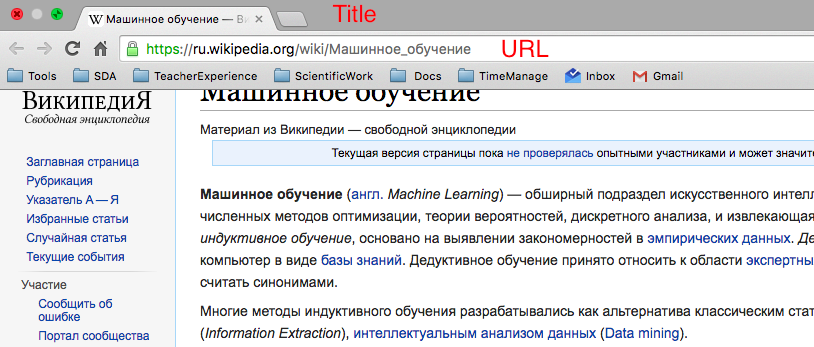
\includegraphics[scale=0.3]{br}
\end{center}

Эти данные хочется использовать для получении прибыли, один из путей монетизации данных это продаже рекламным системам некоторой информации про пользователя -- пол, возраст, доход интересы, имея эту информацию можно персонализировать рекламу для увеличения эффективности рекламной компании. Обучающую выборку при этом можно найти в других сервисах вашей компании, к примеру почте (возраст указывается при регистрации). 

Вам, как специалистам по машинному обучению нужно построить алгоритм предсказания возраста пользователя по его браузерной истории.

\subsection*{Описание Данных и Метрик}

Каждый файл с данными, это csv файл с разделителем \texttt{tab}:
\begin{enumerate}
	\item \texttt{age\_profile\_train} -- user\_id(str), age(int -- traget value)
    \item \texttt{(url\_domain/title\_unify)\_(train/test)} -- user\_id(str), url/title (str), num\_vizits (int)
\end{enumerate}

В качестве метрики используется Mean Squared Error (MSE):
$$MSE(y, \hat{y}) = \frac{1}{N}\sum_i^N (y_i - \hat{y}_i)^2$$

\subsection*{Сдача Задания и Правила Игры}
\begin{enumerate}
	\item Можно использовать любые реализации изученных на курсе моделей
    \item Нужно будет  + прислать отчет в виде ipython notebook с описанием экспериментов
    \item Задание оценивается максимальным баллом если вы
   	\begin{enumerate}
		\item побили baseline + сдали задание вовремя
        \item использовали хотя-бы 2 метода снижения размерности и стекинг моделей
        \item за первые места, как обычно бонусы
	\end{enumerate}
\end{enumerate}

\subsection*{Методические Указания}
  \begin{enumerate}
      \item На сильно разреженной матрице вы не сожмите обучить композиции алгоритмов (RandomForest, Boosting), поэтому стоит посмотреть в сторону линейных моделей и уменьшение размерности пространства. 
      \item В качестве библиотеки для линейных моделей рекомендуется использовать \href{https://github.com/JohnLangford/vowpal_wabbit/wiki}{Vowpal Wabbit}
      \item Для снижения размерности пространства нужно попробовать использовать:
      	\begin{enumerate}
			\item различные матричные разложения SVD, LDA (\href{https://github.com/JohnLangford/vowpal_wabbit/wiki}{Vowpal Wabbit}, \href{https://radimrehurek.com/gensim/}{GenSim})
            \item Hashing Trick -- есть в \href{http://scikit-learn.org/stable/modules/generated/sklearn.feature_extraction.FeatureHasher.html}{SciKit-FeatureHasher}, встроен в \href{https://github.com/JohnLangford/vowpal_wabbit/wiki}{Vowpal Wabbit}
            \item Word2Vec (\href{https://radimrehurek.com/gensim/}{GenSim}) -- обратите внимание, что обучить модель самому может быть:
            \begin{enumerate}
				\item долго -- используйте \href{https://aws.amazon.com/ru/education/awseducate/}{AWS Educate} или пред-обученную модель
               \item тяжело -- уменьшите число параметров за счет снижения размерности векторов
			\end{enumerate}
			\item иные методы учитывающие специфику задачи к примеру гистограмма $p(url | age[00-25])$ для каждого пользователя
        \end{enumerate}
       \item При использовании нейросетевых методов обратите внимание на библиотеку \href{http://lasagne.readthedocs.org/en/latest/index.html}{Lasagne}, 
       \begin{enumerate}
			\item нужно будет внимательно почитать про "convolutional/recurrent neural networks for text"
            \item обратите внимание на EmbeddingLayer, это почти Word2Vec
			\item все эти нейросети работают очень долго используйте \href{https://aws.amazon.com/ru/education/awseducate/}{AWS Educate} нужен инстанс с видеокартой, разумный выбор \texttt{g2.2xlarge}, найдите образ уже с установленными библиотеками
        \end{enumerate} 
        \item Используйте стекинг моделей (несколько уровней регрессий):
        \begin{enumerate}
			\item использовать не больше двух уровней
            \item модель второго уровня обучается на ответах моделей с первого уровня
            \item модель второго уровня должна быть простой(грубой)
            \item модель второго уровня лучше обучать на отдельном hold-out
\end{enumerate}
Будьте аккуратны с кросс-валидацией, не переобучитесь.
\item Вам может помочь, \href{http://www.slideshare.net/antongorokhov/bigdata-week-moscow-2013-case-personalization}{презентация} о решении подобной задачи. 
  \end{enumerate}
  
\vspace{1.2cm}
\emph{Разница между списыванием и помощью товарища иногда едва различима. Мы искренне надеемся, что при любых сложностях вы можете обратиться к семинаристам и с их подсказками самостоятельно справиться с заданием. При зафиксированных случаях списывания (одинаковый код, решение задачи), баллы за задание будут обнулены всем участникам инцидента.}
\end{document}